% =============================================================================
% cof_diagrams.tex — Two-Population Model Diagram (Panel B only)
% Compile:  pdflatex cof_diagrams.tex && open cof_diagrams.pdf
% =============================================================================
\documentclass[border=8pt]{standalone}
\usepackage[dvipsnames,svgnames,x11names]{xcolor}
\usepackage{tikz}
\usepackage{amsmath,amssymb}
\usepackage[scaled]{helvet}
\renewcommand{\familydefault}{\sfdefault}
\usetikzlibrary{
  arrows.meta,
  positioning,
  shapes.geometric,
  decorations.pathreplacing,
  calc,
  fit,
  backgrounds
}

% ─── Color palette ──────────────────────────────────────────────────────────
\definecolor{panelbg}{HTML}{FFFFFF}
\definecolor{canvasbg}{HTML}{F4F5F7}
\definecolor{bordergray}{HTML}{D9E2EC}
\definecolor{textdark}{HTML}{102A43}
\definecolor{textbody}{HTML}{243B53}
\definecolor{textmuted}{HTML}{486581}
\definecolor{smhaRed}{HTML}{F97068}
\definecolor{gfpTeal}{HTML}{2CB1BC}
\definecolor{tailGray}{HTML}{9FB3C8}
\definecolor{foldGreen}{HTML}{2F9E44}
\definecolor{foldGreenLight}{HTML}{D3F9D8}
\definecolor{foldGreenBg}{HTML}{EEFBF2}
\definecolor{nonfoldGrayBg}{HTML}{F1F3F5}
\definecolor{nonfoldGray}{HTML}{BCCCDC}
\definecolor{nonfoldDark}{HTML}{7B8794}
\definecolor{inputBg}{HTML}{EEF2F6}
\definecolor{inputBorder}{HTML}{BCCCDC}

% ─── TikZ styles ────────────────────────────────────────────────────────────
\tikzset{
  panel/.style={
    rounded corners=10pt,
    draw=bordergray, line width=1.2pt,
    fill=panelbg, inner sep=14pt,
  },
  branchpanel/.style 2 args={
    rounded corners=10pt,
    draw=#1, fill=#2, line width=1.5pt,
    inner sep=10pt,
  },
  chip/.style 2 args={
    rounded corners=4pt, fill=#1, text=#2,
    font=\bfseries\sffamily\scriptsize,
    minimum height=16pt, minimum width=38pt,
    inner sep=2pt,
  },
  statebox/.style 2 args={
    rounded corners=8pt,
    draw=#1, fill=#2, line width=1.2pt,
    minimum width=30pt, minimum height=34pt,
    font=\large\bfseries, text=black,
    inner sep=4pt, align=center,
  },
  midarrow/.style={
    -{Stealth[length=3mm,width=2mm]}, line width=1.2pt,
  },
  labeltext/.style={
    font=\small\bfseries, text=black,
  },
  smalltext/.style={
    font=\scriptsize, text=black,
  },
}

\begin{document}
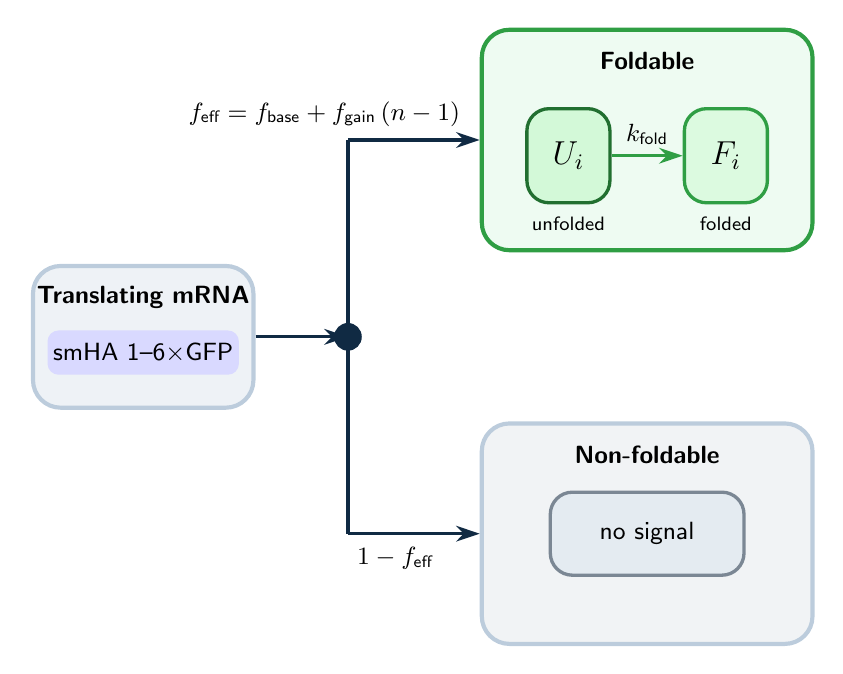
\begin{tikzpicture}

  % ─── Common input (polysome pool) ─────────────────────────────────────
  \node[branchpanel={inputBorder}{inputBg},
        minimum width=2.8cm, minimum height=1.8cm]
    (input) at (0,0) {};

  \node[labeltext, anchor=center] at (0,0.5) {Translating mRNA};

  % Construct chip
  \node[chip={blue!15}{black}, minimum width=65pt,
        font=\small]
    at (0,-0.2) {smHA 1--6$\times$GFP};

  %\node[smalltext, text width=3.2cm, align=center] at (0,-0.7)
  %  {Same mRNA, same elongation};

  % ─── Branch split node ────────────────────────────────────────────────
  \coordinate (split) at (2.6,0);
  \fill[textdark] (split) circle (5pt);
  \draw[midarrow, textdark] (input.east) -- (split);

  % ─── Foldable branch ─────────────────────────────────────────────────
  \node[branchpanel={foldGreen}{foldGreenBg},
        minimum width=4.2cm, minimum height=2.8cm]
    (foldbox) at (6.4,2.5) {};

  \node[labeltext, anchor=center]
    at (6.4,3.5) {Foldable};

  % U_i → F_i scheme
  \node[statebox={foldGreen!70!black}{foldGreenLight}]
    (Ui) at (5.4,2.3) {$U_i$};
  \node[smalltext, below=1pt of Ui] {unfolded};

  \node[statebox={foldGreen}{foldGreenLight!80!white}]
    (Fi) at (7.4,2.3) {$F_i$};
  \node[smalltext, below=1pt of Fi] {folded};

  \draw[midarrow, foldGreen] (Ui) -- node[above, font=\small, text=black]
    {$k_{\text{fold}}$} (Fi);

  % Arrow: split → foldable (vertical line + horizontal arrow)
  \draw[textdark, line width=1.2pt] (split) -- ++(0,2.5);
  \draw[midarrow, textdark] (2.6,2.5) -- (foldbox.west);
  % Fraction label: f_eff = f_base + f_gain·(n-1)
  \node[font=\small, text=black, anchor=south]
    at (2.3,2.55) {$f_{\text{eff}} = f_{\text{base}} + f_{\text{gain}}\,(n-1)$};

  % ─── Non-foldable branch ─────────────────────────────────────────────
  \node[branchpanel={nonfoldGray}{nonfoldGrayBg},
        minimum width=4.2cm, minimum height=2.8cm]
    (nonfoldbox) at (6.4,-2.5) {};

  \node[labeltext, anchor=center]
    at (6.4,-1.5) {Non-foldable};

  % Single box — no kinetic transition modeled
  \node[statebox={nonfoldDark}{nonfoldGray!40!white},
        minimum width=70pt, minimum height=30pt]
    at (6.4,-2.5) {\normalfont\small no signal};

  % Arrow: split → non-foldable (vertical line + horizontal arrow)
  \draw[textdark, line width=1.2pt] (split) -- ++(0,-2.5);
  \draw[midarrow, textdark] (2.6,-2.5) -- (nonfoldbox.west);
  % Fraction label: 1 - f_eff
  \node[font=\small, text=black, anchor=north]
    at (3.2,-2.55) {$1 - f_{\text{eff}}$};

\end{tikzpicture}
\end{document}
